\chapter{Project Involvement}

\section{Electronic Visit Verification}

It was the first and only project I worked on as an intern in Kaz Software.
It has both Mobile and Web application.
I worked on the web application, on front-end.
The design team in Kaz Software made the mock design of the application and I with my teammates brought the design to live.

\begin{center}
    \begin{tabular}{cc}
    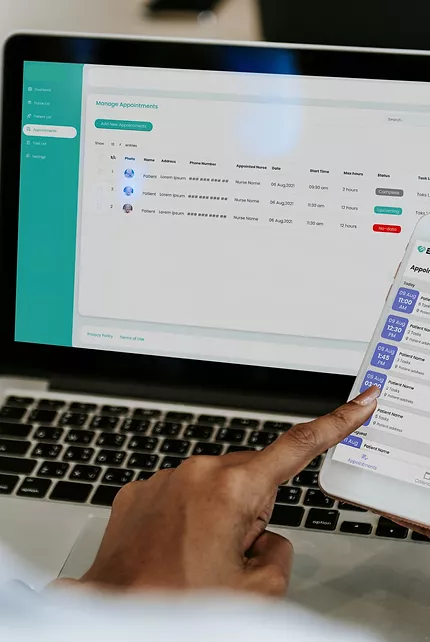
\includegraphics[width=0.475\textwidth]{images/Chapter4/Evv/mock1.png} & 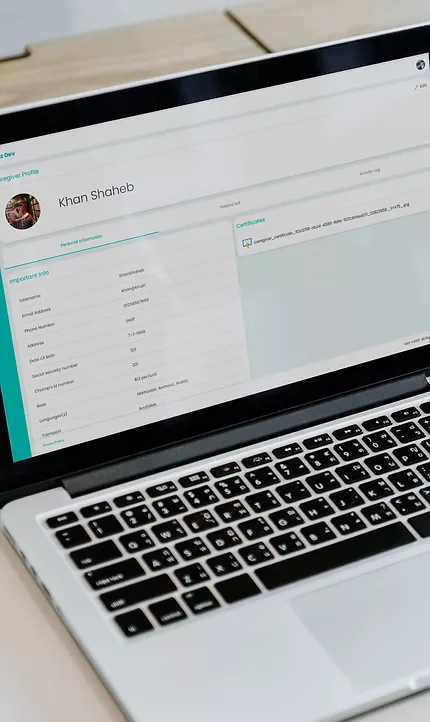
\includegraphics[width=0.4224\textwidth]{images/Chapter4/Evv/mock2.png}
    \end{tabular}
\end{center}

\subsection{Project Overview}

It is a Web and Mobile based application to verify home healthcare visits to ensure patients are not neglected and to cut down on fraudulently documented home visits.
The application is developed around the vendor who can set-up multiple company with each having separate patient and caregiver management.

Due to the 21st Century Cures Act, all care visits provided in the home must be verified electronically — no more pen and paper.
Each state has unique requirements for electronic visit verification which can cause stress and confusion for providers.
This application implement a solution to help the agencies operate more efficiently and advocate for beneficiaries, all while keeping their staff safe. \\

This application offers the most efficient scheduling and EVV capabilities on the market, saving coordinators time, eliminating errors, and making it easy for caregivers to clock in and out.
Using this web-based solution, one can enable more effective workflows across an entire agency environment and automate time-consuming manual tasks.


\subsection{Functionalities}

This application has built-in scheduling and electronic visit verification.
Other system features address HIPAA compliance, documentation, reporting, and billing.
Other features of this application are:

\begin{enumerate}
    \item Capture Documentation at the Point of Service 
    \item Single-Swipe Check-In or Out on Android and iOS devices
    \item Voice or Signature Verification Functionality
    \item GPS and Cellular Visit Tracking
    \item Electronic Attendance Verification
    \item Secure In-Office Messaging
    \item Automated Paper Timesheet Processing
    \item Live Scheduling View
    \item Employee Time and Attendance Management
\end{enumerate}

\subsection{Tools and Technologies}

Tools and technologies used to develop this application are:

\begin{enumerate}
    \item \textbf{Back-end:} .Net Core 3.1, AWS Cognito, Push Notification, Firebase
    \item \textbf{Front-end:} Typescript, ReactJS, Redux, SWR, Axios, RsuiteJS, Bootstrap
    \item \textbf{Database:} Amazon DynamoDB
    \item \textbf{Mobile:} Flutter, Dart, Push Notification
\end{enumerate}

\subsection{My Contribution}

From the first day of my internship I started working in this application.
At first I started working with Ibrahim Bhai and Masum Bhai on the front end using ReactJS and Typescript.
They gave me an overview of the application in the first week and gave me mock design of the application.
And I started working right away.\\

There are two user classes in the front-end web application.
One is for Company admin, another is for Super Admin.
There is one more user class for the mobile application for Caregivers.
In total there were almost 50 pages in the web application and I either designed, implemented, refactored, updated or reviewed each one of them.\\

Later both Ibrahim Bhai and Masum Bhai stopped working on the front-end, I started working with Abdullah Al Jahid and Siana Rizwan, two interns from Dhaka University and Islamic University of Technology respectively.
And during the whole time Pandey Bhai along with Tulshi Bhai, Ibrahim Bhai, Souhardya, developed the backend of the application and Abdullah-Al Foysal developed the mobile application.

\subsection{Project Preview}

Here are some screenshots of the pages I designed:

\setlength{\tabcolsep}{4pt}

\begin{center}
    \begin{tabular}{cc}
    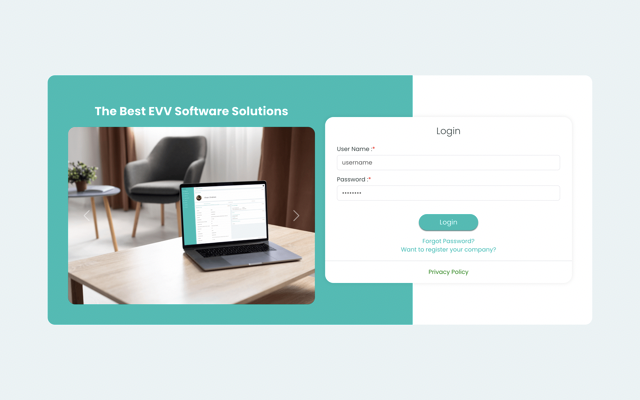
\includegraphics[width=0.475\textwidth]{images/Chapter4/Evv/login_mid.png} & 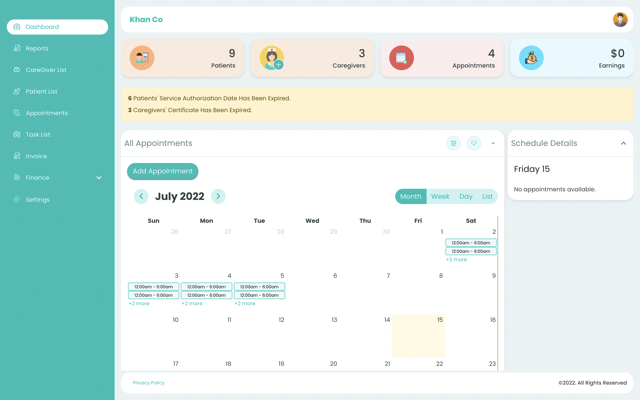
\includegraphics[width=0.475\textwidth]{images/Chapter4/Evv/dashboard_mid.png} \\
    Login Page & Dashboard \\
    \end{tabular}
\end{center}

\begin{center}
    \begin{tabular}{cc}
    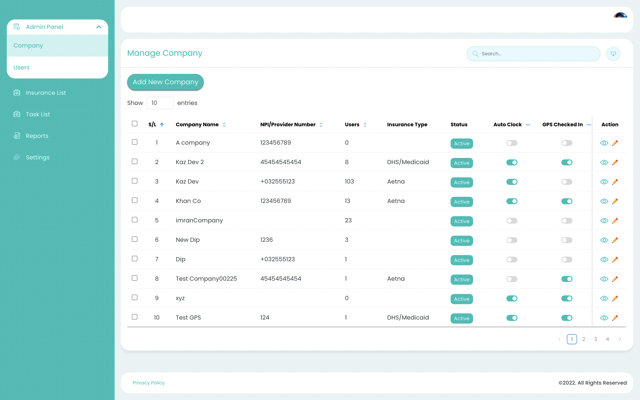
\includegraphics[width=0.475\textwidth]{images/Chapter4/Evv/admin_panel_mid.png} & 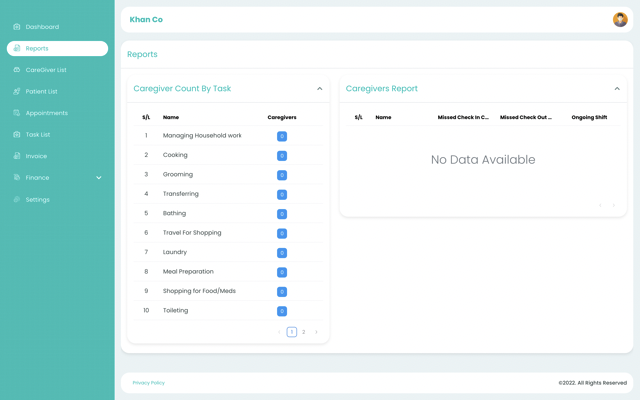
\includegraphics[width=0.475\textwidth]{images/Chapter4/Evv/report_mid.png} \\
    Admin Panel & Reports Page \\
    \end{tabular}
\end{center}

\begin{center}
    \begin{tabular}{cc}
    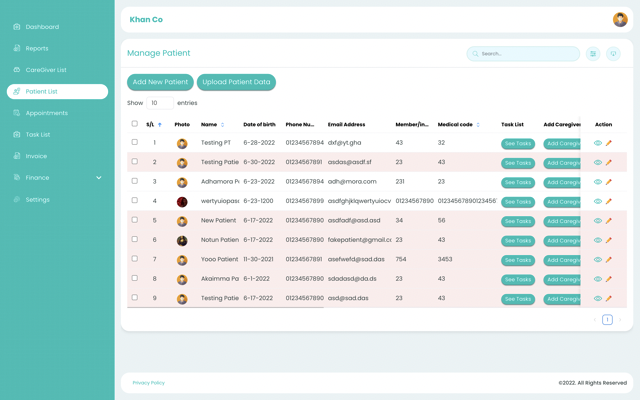
\includegraphics[width=0.475\textwidth]{images/Chapter4/Evv/patient_list_mid.png} & 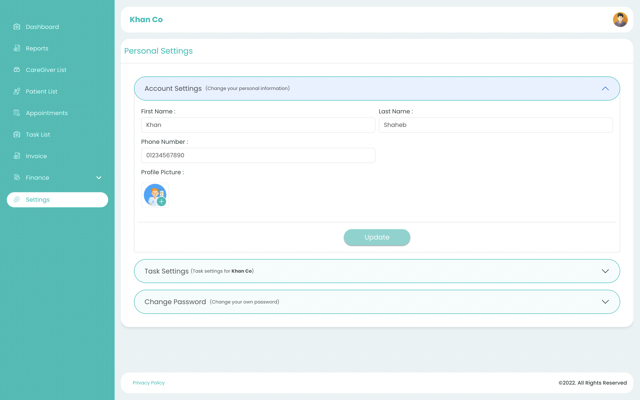
\includegraphics[width=0.475\textwidth]{images/Chapter4/Evv/settings_mid.png} \\
    Patient List & Settings page \\
    \end{tabular}
\end{center}

\begin{center}
    \begin{tabular}{cc}
    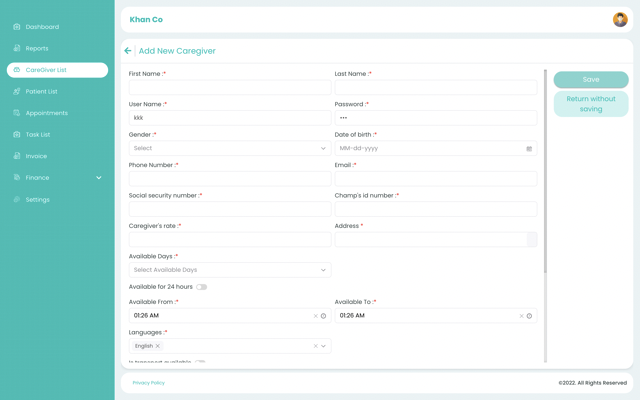
\includegraphics[width=0.475\textwidth]{images/Chapter4/Evv/add_caregiver_mid.png} & 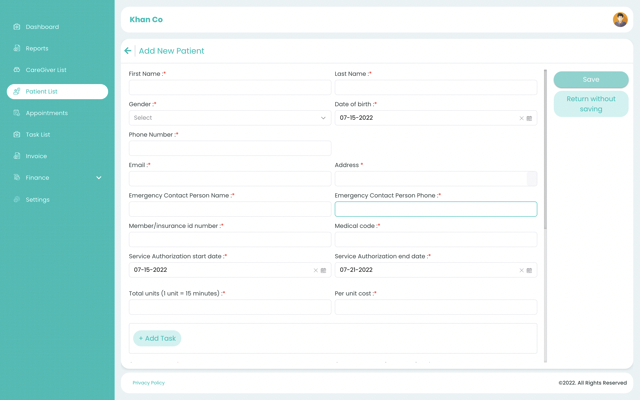
\includegraphics[width=0.475\textwidth]{images/Chapter4/Evv/add_patient_mid.png} \\
    Add Caregiver Page & Add Patient Page \\
    \end{tabular}
\end{center}

\section{Other Involvements}

Beside working on this application, sometimes I solved some problems in other applications and did some research too.

\subsection{Upgrade RegAnalytics}

RegAnalytics is a software and services for regulatory compliance.
It is a combination of more than 6 web applications.
We had to upgrade ReactJS version from 16 and 17 to 18 two parts of the application, TPA and WTA.
I worked with Abdullah Al Jahid during this task.
We had to upgrade the version of ReactJS to 18 then test full application on the new version.
And fix if something does not work properly.

\subsection{Design Nest Publisher}

Nest Publisher is a part of the RegAnalytics application.
It was previously built on a different platform and had a backdated design, and we had to design this application using ReactJS.
The mock design of the application was provided by Design Team in Kaz Software and we had to implement those design.
I worked with Abdullah Al Jahid during this task too.

\subsection{Research and Development}

During my internship did some Research and Development too.
I had to research about how does micro-frontends work and create a proof-of-concept using a javascript package called Single-SPA.
I also had to research about Kubernetes and how to deploy docker containers on Kubernetes.